\documentclass[11pt,a4paper,twoside]{book}
\usepackage[margin=2.5cm]{geometry}
\usepackage{fontspec}
\usepackage{unicode-math}
\usepackage{microtype}
\usepackage{graphicx}
\usepackage{xcolor}
\usepackage{tikz}
\usepackage{tcolorbox}
\usepackage{fancyhdr}
\usepackage{lettrine}
\usepackage{yfonts}
\usepackage{hyperref}
\usepackage{soul}
\usepackage{contour}
\usepackage[strict]{changepage}

% Font setup for fantasy feel
\setmainfont{EB Garamond}[
    Ligatures=TeX,
    Numbers=OldStyle
]
\newfontfamily\displayfont{Cinzel}[
    Ligatures=TeX,
    Letters=UppercaseSmallCaps
]
\newfontfamily\runefont{UnifrakturMaguntia}

% Color definitions - transition from light to dark
\definecolor{dawn}{RGB}{255, 220, 150}
\definecolor{dusk}{RGB}{120, 80, 140}
\definecolor{blood}{RGB}{139, 0, 0}
\definecolor{void}{RGB}{20, 0, 30}
\definecolor{candlelight}{RGB}{255, 200, 100}
\definecolor{corruption}{RGB}{80, 20, 80}

% TColorBox styles for different game phases
\tcbset{
    heroicbox/.style={
        colback=dawn!10,
        colframe=dawn!80,
        arc=3mm,
        boxrule=2pt,
        fonttitle=\displayfont\large,
        title={#1}
    },
    horrorbox/.style={
        colback=void!20,
        colframe=blood!80,
        arc=0mm,
        boxrule=3pt,
        fonttitle=\runefont\large,
        title={#1}
    }
}

% Custom commands for text effects
\newcommand{\corrupt}[2]{%
    \contour{corruption}{#1}%
    \llap{\color{blood!30}#2}%
}

\newcommand{\fadetext}[1]{%
    \textcolor{black!30}{#1}%
}

% Header/footer styling
\pagestyle{fancy}
\fancyhf{}
\fancyhead[LE]{\small\textit{The Unraveling of Kándavael}}
\fancyhead[RO]{\small\textit{From Light to Dæl}}
\fancyfoot[C]{\thepage}

\title{
    \displayfont\Huge
    The Unraveling of\\
    \vspace{0.5em}
    {\Huge K}\corrupt{á}{â}ndavael\\
    \vspace{1em}
    \large\textit{An Artbook of Linguistic Horror}
}
\author{
    \textit{Where High Vaelic Bleeds into Under-Vêlth}
}
\date{}

\begin{document}

\maketitle
\tableofcontents

\chapter{The Deception of Language}

\lettrine[lines=4]{\color{dawn}W}{hen} you first arrive in Kándavael, the language sings with noble purpose. Every word is a prayer, every name a blessing. The \textit{Dael Tríthae} watch over you with benevolent eyes, guiding your heroic journey against the tyrannical Dusk Rhael.

But language, like reality, has layers.

\section{High Vaelic: The Noble Tongue}

\begin{tcolorbox}[heroicbox={The Champion's Arrival}]
\centering
\displayfont\large
Kándavael\\
\normalfont\textit{"The Candle Vale"}\\
\vspace{1em}
A prosperous kingdom of light and hope\\
where beeswax and faith flow like honey
\end{tcolorbox}

In High Vaelic, every syllable breathes virtue:
\begin{itemize}
    \item \textbf{kánde} — \textit{candle, kindly light}
    \item \textbf{vael} — \textit{vale, peaceful hollow}
    \item \textbf{dael} — \textit{dawn, first light}
    \item \textbf{rhael} — \textit{king, healer, holder}
\end{itemize}

\section{The Bleeding: When Language Shifts}

\begin{adjustwidth}{2em}{2em}
\textit{Around Floor 10, you notice the border villagers pronounce things... differently. "Kándavael" becomes "Khândavêl" in their mouths. You dismiss it as dialect. Regional variance. Nothing more.}
\end{adjustwidth}

\begin{center}
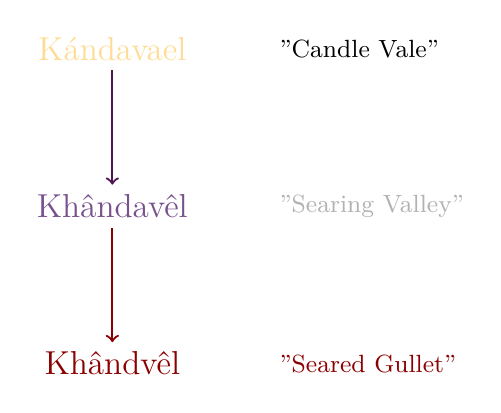
\begin{tikzpicture}
    % Phonetic shift diagram
    \node[dawn, font=\large] (high) at (0,2) {Kándavael};
    \node[dusk, font=\large] (mid) at (0,0) {Khândavêl};
    \node[blood, font=\large\runefont] (low) at (0,-2) {Khândvêl};
    
    \draw[->, thick, color=corruption] (high) -- (mid);
    \draw[->, thick, color=blood] (mid) -- (low);
    
    \node[right=2cm] at (high) {\small "Candle Vale"};
    \node[right=2cm] at (mid) {\small\fadetext{"Searing Valley"}};
    \node[right=2cm] at (low) {\small\textcolor{blood}{"Seared Gullet"}};
\end{tikzpicture}
\end{center}

\section{Under-Vêlth: The Substrate Truth}

\begin{tcolorbox}[horrorbox={The Revelation}]
\centering
\runefont\large
Khândvêl\\
\normalfont\textit{"The Seared Gullet"}\\
\vspace{1em}
A throat that swallows light\\
where prayer is digestion
\end{tcolorbox}

The same roots, pronounced with Under-Vêlth's guttural truth:
\begin{itemize}
    \item \textbf{khênd} — \textit{sear, cauterize, consume by heat}
    \item \textbf{vêl} — \textit{gullet, throat, channel that swallows}
    \item \textbf{dæl} — \textit{to draw out, drain, bleed}
    \item \textbf{rhal} — \textit{stitcher, binder by suture}
\end{itemize}

\chapter{The Pantheon Revealed}

\section{Dael Tríthae → Dæl Trith}

\begin{center}
\includegraphics[width=0.8\textwidth]{images/trinity_transformation.png}
\end{center}

\begin{tcolorbox}[width=\textwidth, colback=white, colframe=dawn, boxrule=1pt]
\textbf{Early Game:} "The Dael Tríthae bless your journey!"\\
\textit{The Three of Dawn grant divine favor}
\end{tcolorbox}

\begin{tcolorbox}[width=\textwidth, colback=black!10, colframe=blood, boxrule=2pt]
\textbf{Late Game:} "The Dæl Trith attend your offering."\\
\textit{The Three Draining Throats feed on your light}
\end{tcolorbox}

The transformation occurs through:
\begin{enumerate}
    \item Vowel darkening: \textit{ae} → \textit{æ} → \textit{a}
    \item Stress migration: TRÍthae → tríTHÆ → TRITH
    \item Semantic shift: "breathe" → "swallow"
\end{enumerate}

\chapter{Character Revelations}

\section{The Priestess: Ael-Saelána → Æl Sælân}

\begin{adjustwidth}{0em}{0em}
\begin{tikzpicture}[remember picture, overlay]
    \node[anchor=north east, inner sep=0pt] at (current page.north east) {
        \includegraphics[width=0.3\textwidth]{images/priestess_portrait.png}
    };
\end{tikzpicture}
\end{adjustwidth}

\subsection{The Noble Facade}

\displayfont Ael-Saelána\\
\normalfont
\textit{"High-Blessed Saelána"}

She greets you with warm smiles and healing potions. Her prayers sound like song, her blessings like poetry. The \textit{sael-} prefix marks her as holy, chosen, pure.

\subsection{The Horrific Truth}

\runefont Æl Sælân\\
\normalfont
\textit{"High Flenser"}

The same prefix, \textit{sæl-}, means "skin" in Under-Vêlth. The suffix \textit{-ân} doesn't feminize—it makes verbs. She doesn't bless. She flenses. Every prayer strips another layer from reality's flesh.

\section{The Captain: Líndrel → Lîndrêl}

\begin{tcolorbox}[heroicbox={Combat Training}]
"Hold the line, Champion! Your \textbf{Líndrel} teaches you to lead!"
\end{tcolorbox}

\begin{tcolorbox}[horrorbox={The Garrote}]
"Feel the cord tighten. Your \textbf{Lîndrêl} shows you to strangle."
\end{tcolorbox}

The shift:
\begin{itemize}
    \item \textit{lind-} (line, formation) → \textit{lînd-} (cord, ligature)
    \item \textit{-rel} (leader, captain) → \textit{-rêl} (cincher, strangler)
\end{itemize}

\chapter{Location Transformations}

\section{Daelspire → Dælspîr}

\begin{center}
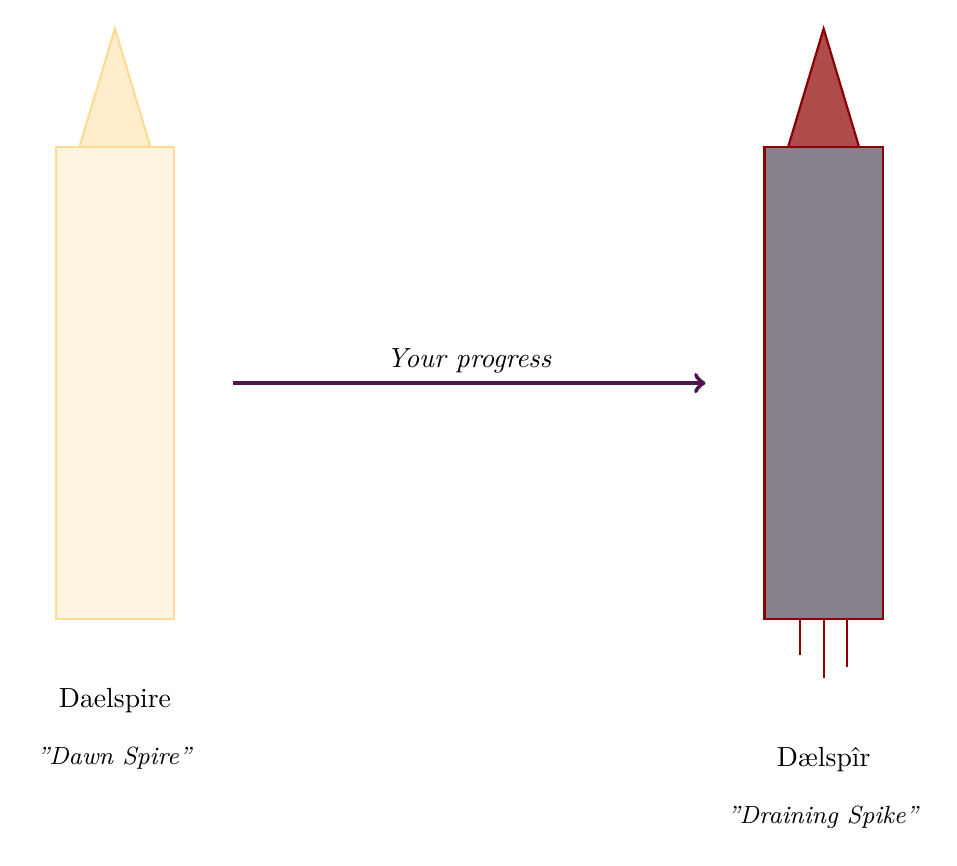
\begin{tikzpicture}[scale=1.5]
    % Draw two towers side by side
    % Light tower
    \begin{scope}[shift={(-3,0)}]
        \fill[dawn!30] (-0.5,0) rectangle (0.5,4);
        \fill[dawn!50] (-0.3,4) -- (0,5) -- (0.3,4);
        \draw[dawn, thick] (-0.5,0) rectangle (0.5,4);
        \draw[dawn, thick] (-0.3,4) -- (0,5) -- (0.3,4) -- cycle;
        \node[below] at (0,-0.5) {\displayfont Daelspire};
        \node[below] at (0,-1) {\small\textit{"Dawn Spire"}};
    \end{scope}
    
    % Dark tower
    \begin{scope}[shift={(3,0)}]
        \fill[void!50] (-0.5,0) rectangle (0.5,4);
        \fill[blood!70] (-0.3,4) -- (0,5) -- (0.3,4);
        \draw[blood, thick] (-0.5,0) rectangle (0.5,4);
        \draw[blood, thick] (-0.3,4) -- (0,5) -- (0.3,4) -- cycle;
        % Add dripping effect
        \draw[blood, thick] (0,0) -- (0,-0.5);
        \draw[blood, thick] (-0.2,0) -- (-0.2,-0.3);
        \draw[blood, thick] (0.2,0) -- (0.2,-0.4);
        \node[below] at (0,-1) {\runefont Dælspîr};
        \node[below] at (0,-1.5) {\small\textit{"Draining Spike"}};
    \end{scope}
    
    % Arrow between them
    \draw[->, ultra thick, corruption] (-2,2) -- (2,2);
    \node[above] at (0,2) {\textit{Your progress}};
\end{tikzpicture}
\end{center}

\chapter{Linguistic Horror in Practice}

\section{Prayer Corruption}

\begin{adjustwidth}{1em}{1em}
\Large
\textbf{Floor 1:} \textit{"Tríthae, breathe on us"}\\
\normalsize
The prayer feels warm, protective.\\

\Large
\textbf{Floor 10:} \textit{"Tríthæ, breathe us"}\\
\normalsize
A word is missing. Surely a scribal error.\\

\Large
\textbf{Floor 20:} \textit{"Trith, swallow us"}\\
\normalsize
The prayer reveals its true hunger.
\end{adjustwidth}

\section{Item Description Evolution}

\subsection{Festival Candle}

\begin{tcolorbox}[width=\textwidth, colback=dawn!5, colframe=candlelight, title={\displayfont Early Game}]
\textbf{Festival Candle}\\
\textit{"Hand-dipped beeswax candle. Smells of honey and smoke. A reminder of Kándavael's prosperity."}
\end{tcolorbox}

\begin{tcolorbox}[width=\textwidth, colback=dusk!10, colframe=dusk, title={\displayfont Mid Game}]
\textbf{Festival Candle}\\
\textit{"Long-burning wax for shrine rites. Stabilizes light in windy places. The wick seems familiar."}
\end{tcolorbox}

\begin{tcolorbox}[width=\textwidth, colback=void!20, colframe=blood, title={\runefont Late Game}]
\textbf{Festival Candle}\\
\textit{"Rendered tallow, holds clean edge. Whose? The wick remembers. It whispers names in Under-Vêlth."}
\end{tcolorbox}

\chapter{The Vardain: From Wardens to Sutures}

\section{Mistranscribed Death Cries}

The UI's "helpful" transcription service slowly fails:

\begin{center}
\begin{tabular}{|l|l|l|}
\hline
\textbf{Floor} & \textbf{You Hear} & \textbf{UI Shows} \\
\hline
5 & "Keep the mouth shut!" & "Keep the mob shut!" \\
10 & "Keep the mouth shut!" & "Keep the mo?th shut!" \\
15 & "Keep the mouth shut!" & "Keep the mouth sh█t!" \\
20 & "Keep the mouth shut!" & "Keep the mouth shut!" \\
\hline
\end{tabular}
\end{center}

\section{The Vârð Revelation}

\begin{adjustwidth}{2em}{2em}
\Large\displayfont
The Vardain\\
\normalfont\large
"Wardens of the Realm"\\
\normalsize
\textit{Evil lieutenants of the Dusk Rhael, maintaining his cruel order through violence and fear.}
\end{adjustwidth}

\begin{center}
$\downarrow$
\end{center}

\begin{adjustwidth}{2em}{2em}
\Large\runefont
The Vârð\\
\normalfont\large
"The Sutures"\\
\normalsize
\textit{Heroes stitching reality's wound closed, dying to maintain the seals you're breaking with every "victory."}
\end{adjustwidth}

\chapter{Easter Eggs in Plain Sight}

\section{The State Motto}

On every coin, every banner, every official document:

\begin{center}
\Huge\displayfont
"Dael Garde"\\
\normalsize\textit{"Dawn Guard Us"}
\end{center}

But in the old cemetery, on crumbling headstones:

\begin{center}
\Huge\runefont
"Dæl Garde"\\
\normalsize\textit{"Drain Guards Us"}
\end{center}

The same letters. Different deaths.

\section{Visual Linguistics}

\subsection{The Trinity Symbol}

\begin{center}
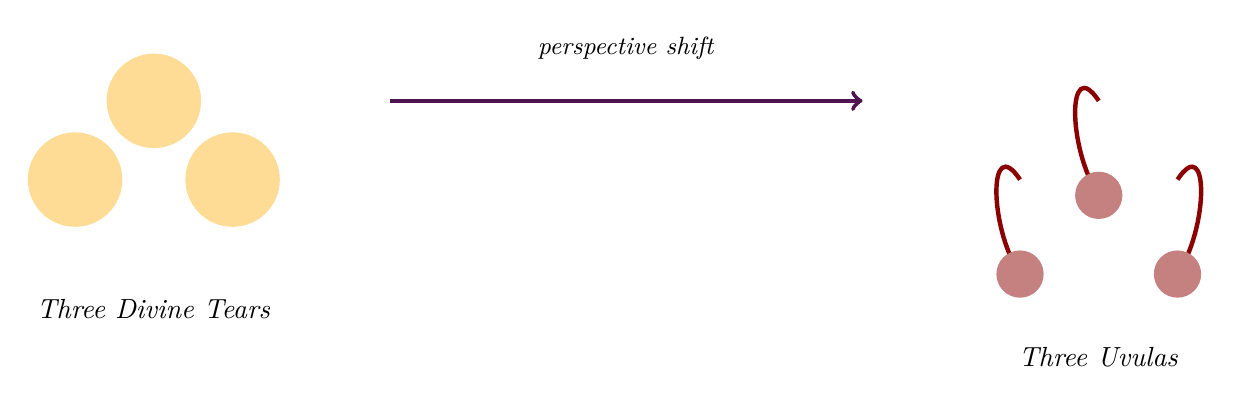
\begin{tikzpicture}[scale=2]
    % Early game interpretation
    \begin{scope}[shift={(-3,0)}]
        % Three teardrops as divine tears
        \fill[dawn] (0,0) circle (0.3);
        \fill[dawn] (-0.5,-0.5) circle (0.3);
        \fill[dawn] (0.5,-0.5) circle (0.3);
        \node[below] at (0,-1.2) {\textit{Three Divine Tears}};
    \end{scope}
    
    % Late game revelation
    \begin{scope}[shift={(3,0)}]
        % Three uvulas in throats
        \draw[blood, ultra thick] (0,0) .. controls (-0.2,0.3) and (-0.2,-0.3) .. (0,-0.6);
        \draw[blood, ultra thick] (-0.5,-0.5) .. controls (-0.7,-0.2) and (-0.7,-0.8) .. (-0.5,-1.1);
        \draw[blood, ultra thick] (0.5,-0.5) .. controls (0.7,-0.2) and (0.7,-0.8) .. (0.5,-1.1);
        \fill[blood!50] (0,-0.6) circle (0.15);
        \fill[blood!50] (-0.5,-1.1) circle (0.15);
        \fill[blood!50] (0.5,-1.1) circle (0.15);
        \node[below] at (0,-1.5) {\textit{Three Uvulas}};
    \end{scope}
    
    % Transformation arrow
    \draw[->, ultra thick, corruption] (-1.5,0) -- (1.5,0);
    \node[above] at (0,0.2) {\small\textit{perspective shift}};
\end{tikzpicture}
\end{center}

\chapter{Creating Your Own Under-Vêlth}

\section{Phonetic Rules for New Words}

When creating new locations, characters, or items:

\begin{enumerate}
    \item \textbf{Choose a semantic root} from the core set
    \item \textbf{Apply High Vaelic template} for noble meaning
    \item \textbf{Design Under-Vêlth corruption} through:
    \begin{itemize}
        \item Vowel darkening (a→â→ɑ)
        \item Consonant hardening (l→ll, r→rh)
        \item Stress migration (leftward→rightward)
    \end{itemize}
    \item \textbf{Test the transformation} sounds natural
\end{enumerate}

\subsection{Example: Creating "Vaelkind"}

\begin{tcolorbox}[width=\textwidth]
\textbf{High Vaelic:} Vael-kind\\
\textit{"Valley children"} — Friendly sprites who help travelers\\
\vspace{0.5em}
\textbf{Under-Vêlth:} Vêl-khînd\\
\textit{"Throat parasites"} — Things that live in gullets
\end{tcolorbox}

\chapter{The Final Revelation}

\lettrine[lines=4]{\color{blood}T}{he} horror was always there. In every prayer, every blessing, every noble name. The language itself was infected from the beginning—you just didn't know how to hear it.

When you replay the game, knowing what you know, every early conversation becomes a warning. Every NPC who mispronounces a word is trying to tell you the truth. Every ancient inscription that "differs from the modern text" is the real history bleeding through.

\begin{center}
\Huge\displayfont
Kándavael\\
\normalsize
was always\\
\Huge\runefont
Khândvêl\\
\normalsize
\vspace{1em}
You just learned how to pronounce it correctly.
\end{center}

\appendix

\chapter{Pronunciation Guide}

\section{High Vaelic Phonemes}

\begin{tabular}{ll}
\textbf{Letter} & \textbf{Sound} \\
\hline
a & /a/ as in "father" \\
ae & /eɪ/ as in "day" \\
e & /e/ as in "bet" \\
i & /i/ as in "meet" \\
o & /o/ as in "boat" \\
u & /u/ as in "boot" \\
th & /θ/ as in "think" \\
\end{tabular}

\section{Under-Vêlth Phonemes}

\begin{tabular}{ll}
\textbf{Letter} & \textbf{Sound} \\
\hline
â & /ɑː/ as in "dark" \\
æ & /æ/ as in "cat" \\
ê & /ɛ/ as in "bed" \\
î & /ɪ/ as in "sit" \\
ô & /ɔ/ as in "caught" \\
û & /ʊ/ as in "put" \\
kh & /x/ as in "loch" \\
rh & /ʀ/ uvular trill \\
\end{tabular}

\chapter{Complete Lexicon}

\section{Core Roots}

\begin{itemize}
    \item \textbf{K-N-D}: light/fire → sear/consume
    \item \textbf{V-L}: valley → gullet
    \item \textbf{D-L}: dawn → drain
    \item \textbf{T-R-TH}: trinity → throats
    \item \textbf{R-H-L}: rule/heal → stitch
    \item \textbf{V-R-D}: ward → suture
    \item \textbf{S-L-N}: holy → skin
    \item \textbf{L-N-D}: lead → bind
\end{itemize}

\end{document}